\documentclass[english,engineering]{wizthesis}

\usepackage[utf8]{inputenc}
\usepackage{float} % H float positioning
\usepackage{xcolor}
\usepackage{enumitem} % enumerate
\usepackage{amsmath, bm}
\usepackage{mathtools}
\usepackage[ruled,vlined]{algorithm2e}
\usepackage{wrapfig}
\usepackage{tikz}

% Set up the thesis
\author{Karol Belina}
\title{Formal grammar\par production rule parsing tool}
\supervisor{dr inż. Zdzisław Spławski}
\fieldofstudy{Computer Science}
\keywords{Parser combinators, context-free grammars, Extended Backus-Naur Form}
\summary{The paper documents the process of designing and implementing a tool
for parsing the production rules of context-free grammars in a textual form. It
discusses the choice of Extended Backus-Naur Form notation over the alternatives
and provides a mathematical model for parsing such a notation. The implemented
parser can turn a high-level specification of a grammar into a parser itself,
which in turn is capable of constructing a parse tree from arbitrary input
provided to the program with the use of parser combinators.}

% Set up the style of code listings (optional)
\setminted{frame=single,breaklines,linenos}
% Set up the bibliography style
\bibliographystyle{acm}

\newcommand{\todo}[1]{{\color{red}[\textbf{TODO} \textit{#1}]}}

\begin{document}

\frontmatter % Disable page and chapter numbering for this section

\maketitle

% '\chapter*' removes the abstract from the table of contents
\chapter*{Abstract}

The thesis presents the design and implementation of an EBNF-based context-free
grammar parsing tool with real-time explanations and error detection. It
discusses the choice of Extended Backus-Naur Form notation over the alternatives
and provides a mathematical model for parsing such a notation. For this purpose,
the official specification of the EBNF from the ISO/IEC 14977 standard has been
examined and transformed into an unambiguous and ready for implementation form.
The thesis proposes a definition of a grammar in the form of an abstract syntax
tree. It describes the process of tokenization --- the act of dividing the
grammar in a textual form into a sequence of tokens --- while taking into
account proper interpretation of Unicode graphemes. The whitespace-agnostic
tokens are then being combined together to form a previously-defined AST with a
technique called \textit{parser combination}. Several smaller helper parsers are
defined, all of which are then combined into more sophisticated parsers capable
of parsing entire terms, productions, and grammars. \todo{coś o regexach w
specjalnych sekwencjach?} The paper defines an algorithm for handling left
recursion in the resulting grammar defined by an AST, as well as a dependency
graph reduction algorithm for determining the starting rule of a grammar. Up to
this stage, any errors encountered in the textual form of a grammar are reported
to the user in a user-friendly format with exact locations of the errors in the
input. The paper thus compares several techniques of storing the locations of
individual tokens and AST nodes for the purposes of error reporting. Further,
the thesis describes a method of testing an arbitrary input against the
constructed grammar to determine if it belongs to the language generated by that
grammar.
\todo{tutaj prawdopodobnie coś o wyjaśnieniach zwracanych przez checker}
The thesis describes the process of creating a simple command line REPL program
to act as a basic tool for interfacing with the grammar parser and checker, but
in order to efficiently use the library, a web-based application is designed on
top of that to serve as a more visual, user-friendly and easily accessible tool.
\todo{tutaj coś o wizualizacjach, edytorze tesktowym i highlightowaniu} The
paper describes the deployment of the application on a static site hosting
service \todo{service workery}, as well as a cross-platform desktop application
with the use of Electron. The designed and implemented system gives the
opportunity to extend it with other grammar specifications.
\todo{poparafrazować ``The thesis describes...''}

\tableofcontents

\mainmatter % Re-enable page and chapter numbering

\chapter{Problem analysis}

\section{Description and motivation} \label{sec:description-and-motivation}

Programming language theory has become a well-recognized branch of computer
science that deals with the study of programming languages and their
characteristics. It is an active research field, with findings published in
various journals, as well as general publications in computer science and
engineering. But besides the formal nature of PLT, many amateur programming
language creators try their hand at the challenge of creating a programming
language of their own as a personal project. It is certainly relevant for a
person to write their own language for educational purposes, and to learn about
programming language and compiler design. However, the language creator must
first of all make some fundamental decisions about the paradigms to be used, as
well as the syntax of the language.

The tools for aiding the design and implementation of the syntax of a language
are generally called \textit{compiler-compilers}. These programs create parsers,
interpreters or compilers from some formal description of a programming
language (usually a grammar). The most commonly used types of
compiler-compilers are \textit{parser generators}, which handle only the
syntactic analysis of the language --- they do not handle the semantic analysis,
not the code generation aspect. The parser generators most generally transform a
grammar of the syntax of a given programming language into a source code of a
parser for that language. The language of the source code for such a parser is
dependent on the parser generator.

Most such tools, however, offer too much complexity and generally have a steep
learning curve for people inexperienced with the topic. Limited availability
makes them less fitted for prototyping a syntax of a language --- they often
require a complex setup for simple tasks, which is not welcoming for new users
\todo{and may lead to...?}. The lack of visualization capabilities shipped with
these tools makes them less desirable for teachers in the theory of formal
languages, who often require such features for educative purposes in order to
present the formulations of context-free grammars in a more visual format.

\section{Goal}

The main goal of this thesis is to design and implement a specialized tool in
the form of an easily accessible web-based application, that serves teachers,
programmers and other kinds of enthusiasts of the theory of formal languages in
the field of discrete mathematics and computer science, in order to formulate
and visualize context-free grammars in the form of the Extended Backus-Naur
Form. The thesis itself will document the entire process of creating such a
project.

\todo{jak projekt pomoże w powyższych problemach?}

In order to achieve the general goal, several sub-goals have been
distinguished, all of which contribute to the main objective as a whole
\begin{itemize}
  \item analysis of existing solutions and applications,
  \item presentation of the theoretical preliminaries of the project,
  \item definition of the outline of the project, including a description of
  the functional and non-functional requirements, the use case diagram, use case
  scenarios, the class diagram, and the user interface prototype,
  \item description of technologies used in the implementation,
  \item implementation of the project,
  \item description of the testing and deployment environments.
\end{itemize}

\section{Scope}

\todo{na pewno zakres? czym to się w ogóle różni?}

\chapter{Theoretical preliminaries}

\section{Formal grammars}

\subsection{Introduction to formal grammars}

\textit{Formal grammar} of a language defines the construction of strings of
symbols from the language's \textit{alphabet} according to the language's
\textit{syntax}. It is a set of so-called \textit{production~rules} for
rewriting certain strings of symbols with other strings of symbols --- it can
therefore generate any string belonging to that language by repeatedly applying
these rules to a given starting symbol \cite{meduna-2014}. Furthermore, a
grammar can also be applied in reverse: it can be determined if a string of
symbols belongs to a given language by breaking it down into its constituents
and analyzing them in the process known as \textit{parsing}.

For now, let's consider a simple example of a formal grammar. It consists of two
sets of symbols: (1) set $N = \{\,S, B\,\}$, whose symbols are
\textit{non-terminal} and must be rewritten into other, possibly non-terminal,
symbols, and (2) set $\Sigma = \{\,a, b, c\,\}$, whose symbols are
\textit{terminal} and cannot be rewritten further. Let $S$ be the start symbol
and set $P$ be the set of the following production rules:
\begin{enumerate}[noitemsep]
  \item $S \rightarrow aBSc$
  \item $S \rightarrow abc$
  \item $Ba \rightarrow aB$
  \item $Bb \rightarrow bb$
\end{enumerate}
To generate a string in this language, one must apply these rules (starting with
the start symbol) until a string consisting only of terminal symbols is
produced. A production rule is applied to a string by replacing an occurrence
of the production rule's left-hand side in the string by that production rule's
right-hand side. The simplest example of generating such a string would be
\begin{equation*}
  S \xRightarrow[2]{} \underline{abc}
\end{equation*}
where $P \xRightarrow[i]{} Q$ means that string $P$ generates the string $Q$
according to the production rule $i$, and the generated part of the string
is underlined.

By choosing a different sequence of production rules we can generate a different
string in that language
\begin{equation*}
\begin{split}
  S & \xRightarrow[1]{} \underline{aBSc} \\
    & \xRightarrow[2]{} aB\underline{abc}c \\
    & \xRightarrow[3]{} a\underline{aB}bcc \\
    & \xRightarrow[4]{} aa\underline{bb}cc
\end{split}
\end{equation*}

After examining further examples of strings generated by these production rules
we may come into a conclusion that this grammar generates the language
$\{\,a^nb^nc^n \mid n \ge 1\,\}$, where $x^n$ is a string of $n$ consecutive $x$'s.
It means that the language is the set of strings consisting of one or more
$a$'s, followed by the exact same number of $b$'s, then followed by the exact
same number of $c$'s.

Such a system provides us with a notation for describing a given
language formally. Such a language is a usually infinite set of finite-length
sequences of terminal symbols from that language.

\subsection{The Chomsky Hierarchy}

\begin{wrapfigure}{R}{0.45\textwidth}
  \centering
  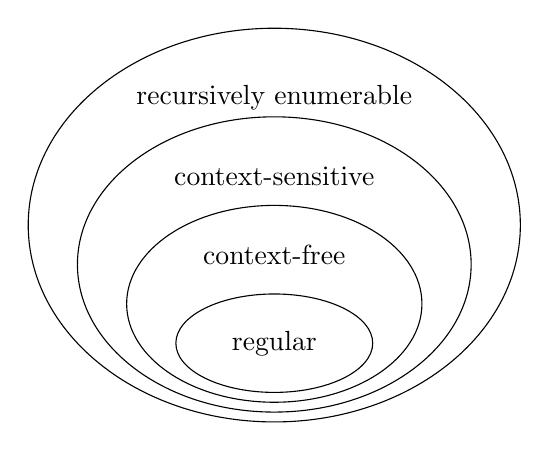
\begin{tikzpicture}[scale=2.5]
    \draw[color=black](0,0) ellipse (1.25 and 1) node at (0, 0.65) {recursively enumerable};
    \draw[color=black](0,-0.2) ellipse (1 and 0.75) node at (0, 0.25) {context-sensitive};
    \draw[color=black](0,-0.4) ellipse (0.75 and 0.5) node at (0, -0.15) {context-free};
    \draw[color=black](0,-0.6) ellipse (0.5 and 0.25) node {regular};
  \end{tikzpicture}
  \caption{The~Chomsky~Hierarchy visualized}
  \label{fig:chomsky-hierarchy}
\end{wrapfigure}

In \cite{chomsky-1956} Chomsky divides formal grammars into four classes and
classifies them in the now called \textit{Chomsky~Hierarchy}. Each class is a
subset of another, distinguished by the complexity.

Type-3 grammars generate the so-called \textit{regular~languages}. As described
in \cite{aho-1990}, regular languages can be matched by
\textit{regular~expressions} and decided by a \textit{finite~state~automaton}.
They are the most restricting kinds of grammars, with its production rules
consisting of a single non-terminal on the left-hand side and a single terminal,
possibly followed by a single non-terminal on the right-hand side. Because of
their simplicity, regular languages are used for lexical analysis of programming
languages \cite{johnson-porter-ackley-ross-1968}.

Type-2 grammars produce \textit{context-free~languages} and can be represented
as a \textit{pushdown~automaton} which is an automaton that can maintain its
state with the use of a stack. \todo{jak w stosie wygląda pamięć}

\subsection{Parsing Expression Grammars}

\todo{\url{https://en.wikipedia.org/wiki/Parsing_expression_grammar}}

\todo{\cite{ford-2004}}

\section{Why EBNF?}

\section{Specification}

\todo{analiza i zmodyfikowanie oficjalnej specyfikacji EBNF}

See appendix \ref{ch:modified-spec}.

\section{Grammar definition}

% \begin{listing}[H]
%   \inputminted[fontsize=\small]{haskell}
%   {listings/ast.hs}
%   \caption{\todo{podpis}}
%   \label{lst:ast}
% \end{listing}

\todo{opis}

\section{Lexical analysis}

\todo{krótko o ``algorytmie'' tokenizacji}

\section{Syntactic analysis} \label{sec:parsing}

\subsection{Methods}

\todo{o różnych metodach i podejściach do parsowania}

\subsection{Parser combination}

\todo{opisanie parser combinatorów w Haskellu \cite{swierstra-2009}
\cite{leijen-2001} \cite{fokker-1995}}

% \begin{listing}[H]
%   \begin{minted}{haskell}
% type Parser a = String -> Maybe (a, String)
%   \end{minted}
%   \caption{\todo{podpis}}
%   \label{lst:parcomb-type}
% \end{listing}

% \begin{listing}[H]
%   \begin{minted}{haskell}
% parse digit "123"
% -- Just ('1', "23")
%   \end{minted}
%   \caption{\todo{podpis}}
%   \label{lst:parcomb-example1}
% \end{listing}

% \begin{listing}[H]
%   \begin{minted}{haskell}
% parse (char 'a') "bcd"
% -- Nothing
%   \end{minted}
%   \caption{\todo{podpis}}
%   \label{lst:parcomb-example2}
% \end{listing}

% \begin{listing}[H]
%   \begin{minted}{haskell}
% parse (multiple (digit <|> letter)) "abc123"
% -- Just ("abc123", "")
%   \end{minted}
%   \caption{\todo{podpis}}
%   \label{lst:parcomb-example3}
% \end{listing}

\subsection{Parser definitions}

\todo{zdefiniowanie ważnych parserów dla EBNF}

\section{Grammar preprocessing}

\subsection{Left recursion handling}

\todo{przedstawienie algorytmu do usuwania lewej rekurencji i wyjaśnienie po co}

% \begin{algorithm}[H]
%   \SetAlgoLined
%   \KwResult{The result}
%   initialization\;
%   \While{condition}{
%     instructions\;
%     \eIf{condition}{
%       instruction1\;
%       instruction2\;
%     }{
%       instruction3\;
%     }
%   }
%   \caption{Name of the algorithm}
% \end{algorithm}

\subsection{Dependency graph reduction}

\todo{przedstawienie algorytmu do wyszukania reguły początkowej}

\section{Grammar processing}

\todo{opisanie sposobu na sprawdzenie czy wejście należy do języka generowanego
przez gramatykę}

\chapter{Analysis of similar solutions}

\section{Coco/R}

\todo{\cite{coco/r}}

\section{ANTLR}

\todo{\cite{antlr}}

\section{Lex and Yacc}

\todo{\cite{lex-yacc}}

\section{PLY}

\todo{\cite{ply}}

\section{Regex101}

\todo{\cite{regex101}}

\chapter{Design}

\section{Requirements}

\subsection{Functional requirements}

\subsection{Non-functional requirements}

\section{Use cases}

\todo{diagram UML}
\todo{scenariusze przypadków użycia}

\section{The architecture}

\subsection{Used technologies}

\todo{Git}
\todo{Rust \cite{rust-book}}
\todo{nom \cite{couprie-2015}}
\todo{Svelte \cite{svelte-docs}}
\todo{Rollup}
\todo{WebAssembly}

\subsection{Class diagram}

\todo{Diagram ``klas''}

\section{Interface prototype}

\todo{obrazki}

\chapter{Implementation}

\section{Environment}

\subsection{Visual Studio Code}

\todo{konfiguracja, rozszerzenia}

\subsection{Git and GitHub}

\todo{w jaki sposób używam Gita, GitHuba, jak używam branchy, issues, PR,
projektów}

\subsection{Cargo}

\todo{konfiguracja Cargo, Clippy}

\subsection{npm}

\subsection{Rollup}

\section{Business logic}

\subsection{Lexer}

\subsection{Parser}

\subsection{Preprocessor}

\subsection{Checker}

\section{Command line application}

\section{Web-based application}

\subsection{Linking the business logic}

\todo{jak się kompiluje Rusta do WebAssembly, czyli wasm-pack}

\subsection{Text editor}

\todo{CodeMirror}

\subsection{Visualizations}

\chapter{Testing}

\section{Automated testing}

\subsection{Business logic testing}

\todo{Cargo test}

\subsection{UI testing}

\todo{Jest}

\section{Manual testing}

\chapter{Deployment}

\section{GitHub Pages}

\section{Electron}

{\backmatter % Disable this chapter number
\chapter{Summary}}

\bibliography{bibliography.bib}

\listoffigures

\listoftables

\listoflistings

\begin{appendices}

\chapter{Modified specification} \label{ch:modified-spec}

\begin{listing}[H]
  \inputminted[fontsize=\small]{lexers/ebnf_lexer.py:EbnfLexer -x}
  {listings/specification.ebnf}
  \caption{Modified version of the EBNF language specification defined in
  \cite{iso-14977}}
  \label{lst:specification}
\end{listing}

\end{appendices}

\end{document}
